   
\documentclass[a4paper,11pt,oneside,article]{memoir}
\renewcommand{\baselinestretch}{1.05}
\usepackage{amsmath,amsthm,verbatim,amssymb,amsfonts,amscd, graphicx}
\usepackage{graphics}
\usepackage[utf8]{inputenc}
\usepackage[danish]{babel}
\topmargin0.0cm
\headheight0.0cm
\headsep0.0cm
\oddsidemargin0.0cm
\textheight23.0cm
\textwidth16.5cm
\footskip1.0cm
\theoremstyle{plain}
\newtheorem{theorem}{Theorem}
\newtheorem{corollary}{Corollary}
\newtheorem{lemma}{Lemma}
\newtheorem{proposition}{Proposition}
\newtheorem*{surfacecor}{Corollary 1}
\newtheorem{conjecture}{Conjecture} 
\newtheorem{question}{Question} 
\theoremstyle{definition}
\newtheorem{definition}{Definition}

\begin{document}

\frontmatter

\title{Latex}

\author{Kristian}

\maketitle

\clearpage

\mainmatter

\chapter{Brug af LaTex}

\begin{enumerate}

 \item Åben Template.tex med texmaker.
 
 \item Tryk F1, og texmaker begynder en "quick build". Du burde nu se et vindue med din pdf, ellers tryk F1 igen.
 
 \item Over i din tex fil, vil du se \textbackslash title \{ Latex \} . Erstat "Latex" med "Mit første latex dokument" og tryk F1.
 
 \item Du kan kan gøre det samme med \textbackslash author \{ mit navn \} og tryk F1 igen. 
 
\end{enumerate}

(Du behøver ikke trykke F1 efter hver lille ændring) 


\chapter{Layout}

\section{Sections og subsections}

Latex består af kapitler og sektioner (og derunder undersektioner og underundersektioner). Formatet er det samme, $\backslash chapter \{ Something \}$, Hvor "Something" er navnet på din afsnit. Prøv at indsætte $\backslash chapter \{ Something \}$ under $ \backslash maketitle$ i din tex dokument og tryk F1. \\
\\
Du kan også lave afsnit med $\backslash section \{ Something else \}$. Prøv at indsætte 
$\backslash section \{ Something else \}$ under $\backslash chapter \{ Something \}$ i din tex dokument og tryk F1. \\
\\
Under $\backslash section \{ Something else \}$ kan du skrive din tekst til afsnitet. Prøv at skrive en lille tekst, og derefter compile med F1.\\
\\
Du kan ligeledes lave underafsnit med $\backslash subsection \{Something \}$ og underunder afsnit med $\backslash subsubsection \{Something \}$. Du behøver ikke lave afsnit eller underafsnit for at skrive brød tekst, men det ser bedre ud.

\section{Newpage og newline}

Hvis du gerne vil starte på en ny side, så skriv $\backslash newpage$.

Ønsker du at lave en ny side, hvor floats (billeder, tabeller etc.) ikke følger med fra de forrige sider, bruger du $\backslash clearpage$. \\

$\backslash \backslash$ efter en linie tekst giver en newline.

\newpage

\chapter{Billeder/tabeller}

\section{Import billeder}

\begin{enumerate}

	\item Find et billede, du gerne vil indsætte, og læg det i samme mappe som din tex fil.

	\item Under din lille tekst fra forrige øvelse indsæt $\backslash includegraphics[scale=1]{pic.png}$
	
	\item Erstat pic.png med navnet på dit billede (husk at tilføre fil- typen på dit billede som vist i 		  eksemplet) 
	
	\item Scale sætter hvor stort billedet skal være, Så scale=0.5 sætter billedet til halv størrelse.

\end{enumerate}


\section{Tabel}

Skriv en sandhedstabel for en AND-gate. \\
\\
Brug http://en.wikibooks.org/wiki/LaTeX til at finde ud af hvordan tabeller laves.

\chapter{Matematik}

Matematiske formler kan skrives på flere forskellige måder. \$ math formel \$ giver et "matematikfelt" in-line, dvs det kan skrives i brødteksten. $\backslash begin \{ displaymath \}$ giver et matematikfelt på sin egen linie og i midten. $\backslash begin \{ equation \}$ gør ca det samme som $displaymath$, men giver linien et nummer, som man kan sætte en label på med $\backslash label \{something \}$ og derefter referere til med $\backslash ref \{something \}$. Indskriv \\
 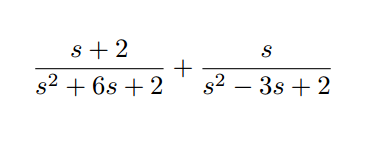
\includegraphics[scale=1]{../lektion/math.png} \\
i latex vha. http://en.wikibooks.org/wiki/LaTeX/Mathematics.


\end{document}